\documentclass[12pt, titlepage]{article}

\usepackage{fullpage}
\usepackage[round]{natbib}
\usepackage{multirow}
\usepackage{booktabs}
\usepackage{tabularx}
\usepackage{graphicx}
\usepackage{float}
\usepackage{hyperref}
\hypersetup{
    colorlinks,
    citecolor=black,
    filecolor=black,
    linkcolor=red,
    urlcolor=blue
}
\usepackage[round]{natbib}

\newcounter{acnum}
\newcommand{\actheacnum}{AC\theacnum}
\newcommand{\acref}[1]{AC\ref{#1}}

\newcounter{ucnum}
\newcommand{\uctheucnum}{UC\theucnum}
\newcommand{\uref}[1]{UC\ref{#1}}

\newcounter{mnum}
\newcommand{\mthemnum}{M\themnum}
\newcommand{\mref}[1]{M\ref{#1}}

\title{SE 3XA3: Software Requirements Specification\\ ohm}

\author{Team 4, Ohm
		\\ Jonathan Brown, brownjs2
		\\ Graeme Crawley, crawleg
		\\ Ryan Marks, marksr2
}

\date{\today}

%% Comments

\usepackage{color}

\newif\ifcomments\commentstrue

\ifcomments
\newcommand{\authornote}[3]{\textcolor{#1}{[#3 ---#2]}}
\newcommand{\todo}[1]{\textcolor{red}{[TODO: #1]}}
\else
\newcommand{\authornote}[3]{}
\newcommand{\todo}[1]{}
\fi

\newcommand{\wss}[1]{\authornote{blue}{SS}{#1}}
\newcommand{\ds}[1]{\authornote{red}{DS}{#1}}
\newcommand{\mj}[1]{\authornote{red}{MSN}{#1}}
\newcommand{\cm}[1]{\authornote{red}{CM}{#1}}
\newcommand{\mh}[1]{\authornote{red}{MH}{#1}}

% team members should be added for each team, like the following
% all comments left by the TAs or the instructor should be addressed
% by a corresponding comment from the Team

\newcommand{\tm}[1]{\authornote{magenta}{Team}{#1}}


\begin{document}


\begin{table}[hp]
\caption{Revision History} \label{TblRevisionHistory}
\begin{tabularx}{\textwidth}{llX}
\toprule
\textbf{Date} & \textbf{Developer(s)} & \textbf{Change}\\
\midrule
11/13/2016 & Ryan M, Jonathan B, Graeme C & Initial Revision\\
11/18/2016 & Ryan M, Jonathan B, Graeme C & Second Revision\\
12/04/2016 & Graeme C & Third Revision\\
\bottomrule
\end{tabularx}
\end{table}


\newpage
\pagenumbering{roman}
\tableofcontents
\listoftables
\listoffigures



\newpage

\pagenumbering{arabic}

\section{Introduction}
\subsection{Overview}
The resistance scanner project is the re-implementation of an open-source software application that allows a user to scan a resistor using their camera and read an on screen value representing the resistance of that resistor.

\subsection{Context}
\par This document is the Module Guide (MG). The Module Guide, written after the SRS, is used as an outline for the implementation of all functional and nonfunctional specified in the SRS. This is done by the decomposition of the system into modules, showing it's structure and design. A brief explanation of each module is given and the requirements outlined in the SRS are directly mapped to their modular implementations. An explanation of the relationships between each module are also given. This is useful both for developers and maintainers as it allows them to more easily identify parts of the software.
\par For a more detailed description of the individual components of the system, the MIS is used to explain the semantics and syntax of the member functions of the classes used in the implementation of the modules.

\subsection{Design Principles}
This project implements the design principles of Single Responsibility, Separation of Concerns and Least Knowledge.
\begin{itemize}
\item \textbf{Single Responsibility:} Each module should only be responsible for the completion of one task.
\item \textbf{Separation of Concerns:} Requirements should be satisfied by as few modules as possible and large degrees of interdependence avoided. 
\item \textbf{Principle of Least Knowledge:} Each module should be implemented with as little knowledge of the other modules of the system as possible.
\end{itemize}

\subsection{Document Structure}
The document structure is as follows:
\begin{itemize}
\item Section 2 lists Anticipated and Unlikely Changes to the system’s implementation. This list is used for the Traceability Matrices later in the document.
\item Section 3 details the explains the Module Hierarchy as well as gives a list of all modules present in the design. 
\item Section 4 explains the Connection Between Requirements and Design, which details how the software requirements are related to the modules.
\item Section 5 provides the Module Decomposition, detailing the module name, secret, and service/responsibility for each module.
\item Section 6 provides the Traceability Matrices. The first matrix connects the requirements to the modules in order to all future developers to better understand which parts of the system fulfill which requirements. The second matrix connects anticipated changes from Section 2 to the modules.
\item Section 7 provides the Uses Hierarchy for the project, which shows the uses relations between modules.
\end{itemize}

\section{Anticipated and Unlikely Changes} \label{SecChange}

\subsection{Anticipated Changes} \label{SecAchange}
\begin{description}
\item[\refstepcounter{acnum} \actheacnum \label{acInput}:] The method of retrieving input images (Camera/Static Image).
\item[\refstepcounter{acnum} \actheacnum \label{acAxis}:] The method of determining the axis of a resistor.
\item[\refstepcounter{acnum} \actheacnum \label{acPlatform}:] The platform of the application (Desktop to Mobile).
\end{description}

\subsection{Unlikely Changes} \label{SecUchange}
\begin{description}
\item[\refstepcounter{ucnum} \uctheucnum \label{ucIO}:] The format of the output data.
\item[\refstepcounter{ucnum} \uctheucnum \label{ucInput}:] The method used to scan the bands resistor.
\item[\refstepcounter{ucnum} \uctheucnum \label{ucInput}:] The method used to get colours from the bands of the resistor.
\item[\refstepcounter{ucnum} \uctheucnum \label{ucInput}:] The method used to calculate values from the resistor colours.
\item[\refstepcounter{ucnum} \uctheucnum \label{ucInput}:] The content of the output.
\end{description}

\section{Module Hierarchy} \label{SecMH}

This section provides an overview of the module design. Modules are summarized
in a hierarchy decomposed by secrets in Table \ref{TblMH}. The modules listed
below, which are leaves in the hierarchy tree, are the modules that will
actually be implemented.

\begin{table}[h]
\centering
\label{my-label}
\begin{tabular}{cl}
\hline
\multicolumn{1}{l}{\textbf{Module Number}} & \textbf{Module Name}    \\ \hline
\textbf{\refstepcounter{mnum} \mthemnum \label{mCI}}                                & Camera Input Module     \\ \hline
\textbf{\refstepcounter{mnum} \mthemnum \label{mII}}                                & Image Input Module      \\ \hline
\textbf{\refstepcounter{mnum} \mthemnum \label{mUI}}                                & User Interface Module   \\ \hline
\textbf{\refstepcounter{mnum} \mthemnum \label{mRID}}                                & Resistor ID Module      \\ \hline
\textbf{\refstepcounter{mnum} \mthemnum \label{mBL}}                                & Band Location Module    \\ \hline
\textbf{\refstepcounter{mnum} \mthemnum \label{mCM}}                                & Colour Mapping Module   \\ \hline
\textbf{\refstepcounter{mnum} \mthemnum \label{mVC}}                                & Value Calculator Module \\ \hline
\end{tabular}
\end{table}

\begin{table}[h!]
\centering
\begin{tabular}{p{0.3\textwidth} p{0.6\textwidth}}
\toprule
\textbf{Level 1} & \textbf{Level 2}\\
\midrule

{Hardware-Hiding Module} 
& Camera Input Module\\
& Image Input Module \\
\midrule

\multirow{1}{0.3\textwidth}{Behaviour-Hiding Module}
& User Interface Module\\
\midrule

\multirow{4}{0.3\textwidth}{Software Decision Module}
& Resistor ID Module \\
& Band Location Module \\
& Colour Mapping Module \\
& Value Calculator Module\\
\bottomrule

\end{tabular}
\caption{Module Hierarchy}
\label{TblMH}
\end{table}



\section{Connection Between Requirements and Design} \label{SecConnection}
\par The system was designed to satisfy the requirements defined in the SRS. In order to make the system easier to implement on both Desktop and Android, it was written using Java and lacks on-screen buttons. The simple user interface also makes it easier to operate and removes any language requirement. OpenCV was chosen as the image processing library due to its availability, in-depth documentation, and broad functionality. OpenCV allows the system to display text, and read images to identify a resistor using two points. 
The system was designed to have all data and functionality stored in the app to avoid the need for internet access. This, in addition to the fact that the app is broken down into modules to avoid complexity, allows it to be built for durability, removing the need to maintain after launch or require live support. The application's modularity is key when dealing with an algorithmically complex problem as modifications to one part of the algorithmic process should not cause issues in other parts.
\par The Hardware-Hiding Modules are useful in making the application multi-platform as it allows the rest of the system to run independent of the hardware. The User Interface Module is responsible for the fulfillment of the usability requirements. Finally, the Software Decision modules must adhere to the performance requirements, ensuring fast performance and high accuracy.

\section{Module Decomposition} \label{SecMD}

The \emph{Secrets} field in a module decomposition is a brief statement of the design decision hidden by the module. 
The \emph{Services} field specifies \emph{what} the module will do without documenting \emph{how} to do it. 
For each module, a suggestion for the implementing software is given under the \emph{Implemented By} title. 
If the entry is \emph{OS}, this means that the module is provided by the operating system or by standard programming language libraries.
Also indicate if the module will be implemented specifically for the software.
Only the leaf modules in the hierarchy have to be implemented. 
If a dash (\emph{--}) is shown, this means that the module is not a leaf and will not have to be implemented. 

\subsection{Hardware Hiding Modules}

\begin{description}
\item[Secrets:] System Camera or File System
\item[Services:] Provides input frames to the modules involved in image processing (M4, M5).
\item[Implemented By:] --
\end{description}

\subsubsection{Camera Input Module (\mref{mCI})}
\begin{description}
\item[Secrets:] Camera Hardware
\item[Services:] Provides images produced by the camera in displayable formats and as a matrix of RGB vectors.
\item[Implemented By:] Operating System \& OpenCV
\end{description}

\subsubsection{Image Input Module (\mref{mII})}
\begin{description}
\item[Secrets:] File System
\item[Services:] Provides images stored locally in displayable formats and as a matrix of RGB vectors.
\item[Implemented By:] Operating System
\end{description}

\subsection{Behaviour-Hiding Module}

\begin{description}
\item[Secrets:]  Combination and use of Software Decision modules.
\item[Services:] Describes the behaviour of the application. Acts as a bridge between the Hardware Hiding and Software Decision modules.
\item[Implemented By:] --
\end{description}

\subsubsection{User Interface Module (\mref{mUI})}

\begin{description}
\item[Secrets:] View and View Controller
\item[Services:] Displays the results of any calculations performed by the software decision module and allows for user input.
\item[Implemented By:] ohm
\end{description}

\subsection{Software Decision Module}

\begin{description}
\item[Secrets:] The algorithms and data structures used to perform the analysis of input frames.
\item[Services:] Computes the resulting resistance based on some input image produced by the Hardware Hiding modules.
  % Changes in these modules are more likely to be motivated by a desire to
  % improve performance than by externally imposed changes.
\item[Implemented By:] --
\end{description}

\subsubsection{Resistor ID Module (\mref{mRID})}

\begin{description}
\item[Secrets:] Method of Body and Axis Identification
\item[Services:] Provides the location of the main axis of the resistor for further processing.
\item[Implemented By:] ohm \& OpenCV
\end{description}

\subsubsection{Band Location Module (\mref{mBL})}

\begin{description}
\item[Secrets:] Band Detection and Sampling Method
\item[Services:] Provides the colours and relative locations of each band of the resistor.
\item[Implemented By:] ohm
\end{description}

\subsubsection{Colour Mapping Module (\mref{mCM})}

\begin{description}
\item[Secrets:] Algorithm to map sampled colours to known possible colours a resistor can take on.
\item[Services:] Produces the most likely real life colour of a band and it's value used in the computation of a resistor value.
\item[Implemented By:] ohm
\end{description}

\subsubsection{Value Calculator Module (\mref{mVC})}

\begin{description}
\item[Secrets:] Method of calculating resistance.
\item[Services:] Calculates the resistance of the resistor based on the input provided by M6.
\item[Implemented By:] ohm
\end{description}

\newpage
\section{Traceability Matrix} \label{SecTM}

This section shows two traceability matrices: between the modules and the
requirements and between the modules and the anticipated changes.

% the table should use mref, the requirements should be named, use something
% like fref
\begin{table}[H]
\centering
\begin{tabular}{p{0.2\textwidth} p{0.6\textwidth}}
\toprule
\textbf{Req.} & \textbf{Modules}\\
\midrule
FR1 & \mref{mUI}  \\
FR2 & \mref{mRID}, \mref{mBL}, \mref{mCM}, \mref{mVC}\\
NF1 &  \mref{mUI}  \\
NF2 & \mref{mUI}  \\
NF3 & \mref{mCI}, \mref{mII}, \mref{mUI}, \mref{mRID}, \mref{mBL}, \mref{mCM}, \mref{mVC}\\
NF4 & \mref{mUI}  \\
NF5 & \mref{mCI}, \mref{mII}, \mref{mUI}, \mref{mRID}, \mref{mBL}, \mref{mCM}, \mref{mVC}\\
NF6 & \mref{mCI}, \mref{mII}, \mref{mUI}, \mref{mRID}, \mref{mBL}, \mref{mCM}, \mref{mVC}\\
NF7 & \mref{mII}, \mref{mRID}, \mref{mBL}, \mref{mCM}, \mref{mVC}\\
NF8 & \mref{mBL}, \mref{mCM}, \mref{mVC}\\
NF9 & \mref{mRID}, \mref{mBL}, \mref{mCM}, \mref{mVC}\\
NF10 & \mref{mUI}  \\
NF11 & \mref{mCI}, \mref{mII}, \mref{mUI}, \mref{mRID}, \mref{mBL}, \mref{mCM}, \mref{mVC}\\
NF12 & \mref{mCI}, \mref{mII}, \mref{mUI}, \mref{mRID}, \mref{mBL}, \mref{mCM}, \mref{mVC}\\
NF13 & \mref{mCI}, \mref{mII}, \mref{mUI}, \mref{mRID}, \mref{mBL}, \mref{mCM}, \mref{mVC}\\
NF14 & \mref{mCI}, \mref{mII}, \mref{mUI}, \mref{mRID}, \mref{mBL}, \mref{mCM}, \mref{mVC}\\
NF15 & \mref{mCI}, \mref{mII}, \mref{mUI}, \mref{mRID}, \mref{mBL}, \mref{mCM}, \mref{mVC}\\
NF16 & \mref{mCI}, \mref{mII}, \mref{mUI}, \mref{mRID}, \mref{mBL}, \mref{mCM}, \mref{mVC}\\
NF17 &\mref{mUI}  \\
\bottomrule
\end{tabular}
\caption{Trace Between Requirements and Modules}
\label{TblRT}
\end{table}

\begin{table}[H]
\centering
\begin{tabular}{p{0.2\textwidth} p{0.6\textwidth}}
\toprule
\textbf{AC} & \textbf{Modules}\\
\midrule
\acref{acInput} & \mref{mII}\\
\acref{acAxis} & \mref{mRID}\\
\acref{acPlatform} & \mref{mCI}, \mref{mII}, \mref{mUI} \\
\bottomrule
\end{tabular}
\caption{Trace Between Anticipated Changes and Modules}
\label{TblACT}
\end{table}

\section{Use Hierarchy Between Modules} \label{SecUse}

\begin{figure}[H]
\centering
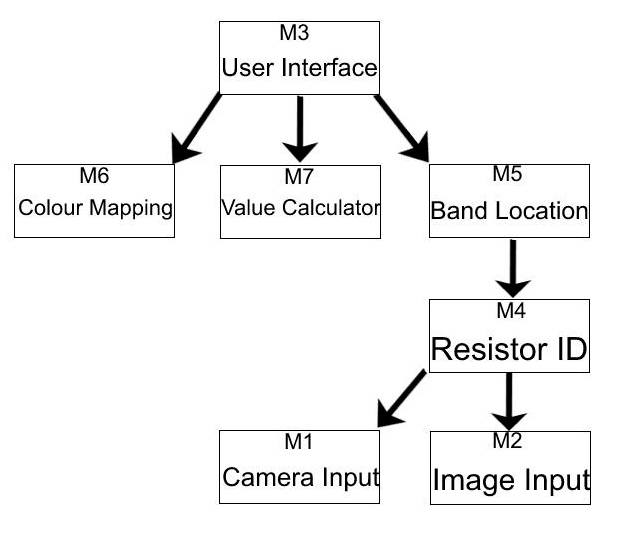
\includegraphics[width=0.7\textwidth]{useshierarchy}
\caption{Use hierarchy among modules}
\label{FigUH}
\end{figure}

\section{Schedule}
Please view the Gantt Chart in the Project Schedule directory of this repository.

%\section*{References}

\bibliographystyle {plainnat}
\bibliography {MG}

\end{document}